\section{Dynamic Compensators and Stability Margins}

\subsection{Stability Margins}

Gain margin: factor by which the gain can be rained before a system becomes unstable.
An uncertainty that may affect the gain of the system could be inertia.


Phase margin: The amount by which the phase can be increased before the system becomes unstable. (exceeds $-180 ^\circ$)
An uncertainty that may affect the phase of the system could be communication delays betweeen a controller and a sensor.

For a system to be robust the gain margin should be 3 to 6dB and the phase margin
should be $30^\circ$ to $45^\circ$.

Remember when finding the phase and gain margin one should use the loop gain $L(s)$.
The phase margin can be found on a bode plot by looking at the phase at the frequency
where the gain is 0dB. The phase margin is then $180^\circ$ minus the phase at that frequency.
The gain margin is the gain at the frequency where the phase is $-180^\circ$.


\begin{center}
	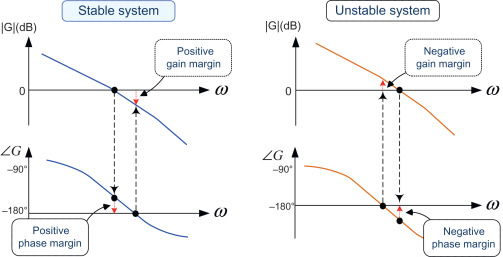
\includegraphics[width=0.7\textwidth]{Images/margin.jpg}
\end{center}


Neutral stability for loop gain $L(s)$ is when $L(s) = -1$. This is the same as a gain of 1 and a phase of $-180^\circ$.


\textbf{Nyquist}

When we encircle -1 then you will have a pole in the right half plane. From the plot below
it can be seen that the plot can be rotated the degrees that the phase margin is.
The gain margin can be interpreted as seen on the figure below.

\begin{center}
	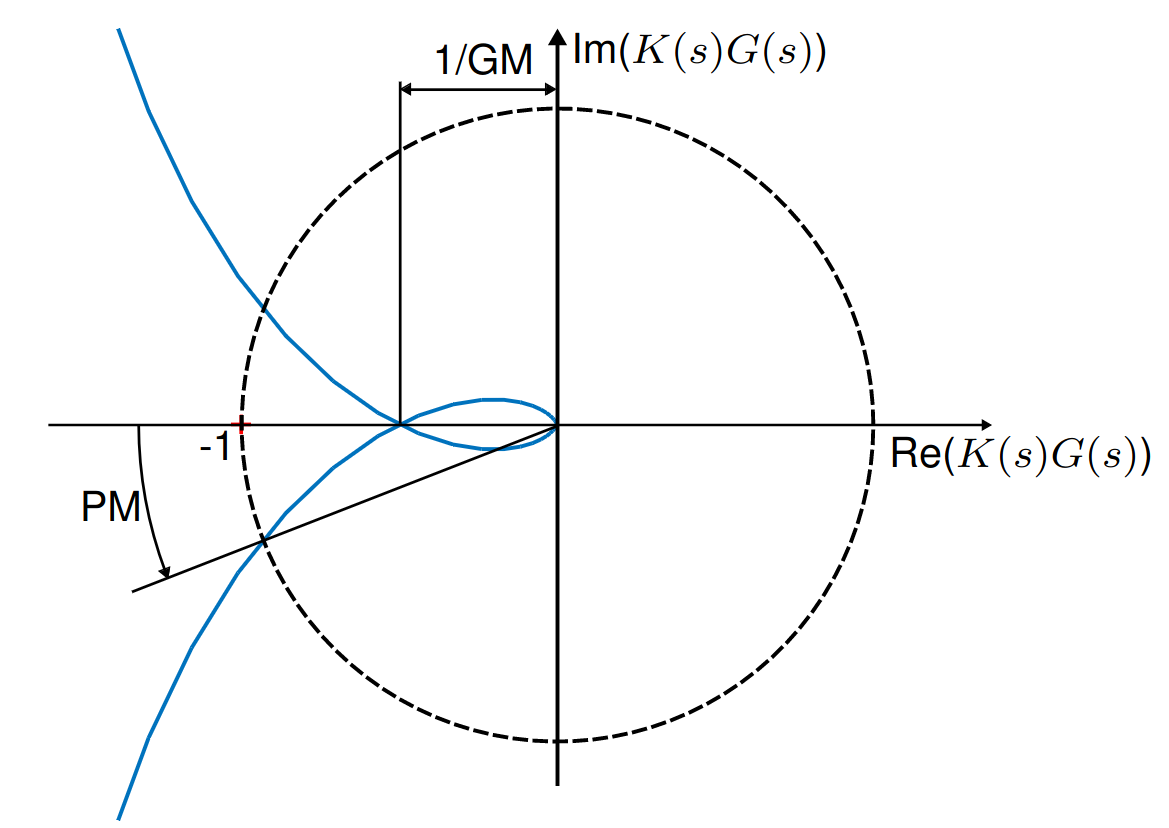
\includegraphics[width=0.5\textwidth]{Images/nyquist.png}
\end{center}

The advantage of using a nyquist plot compared to a bode plot is that you can see
the phase and gain margin at the same time.

\subsection{Dynamic compensation}

Lead compensator is equivalent to a d-part for a PID controller.
A lead compensator has a positive phase. A lead compensater decreases
the rise time and overshoot.

Lag compensator is equivalent to an i-part for a PID controller.
The lag controller improves the steady state tracking.

Both compensators are given by the transfer function:

$$ D(s) = K \frac{s + z}{s + p} $$
Where $z$ and $p$ are the zero and pole of the transfer function respectively.

\begin{itemize}
	\item {If $z<p$, then $D(s)$ is called a lead compensation}
	      \item{If $z>p$, then $D(s)$ is called a lag compensation}
\end{itemize}

\subsubsection{Lead compensation}

Used for dynamic properties such as rise time, overshoot and settling time. It has relation
to the phase margin, where we can lift the phase margin by adding a lead compensator.

A lead compensation is given by:
$$D(s) = \frac{Ts+1}{\alpha Ts+1}$$
and $1/\alpha$ is called the lead ratio.

We have the following properties:
$$\omega_{max} = \frac{1}{T\sqrt{\alpha}} = \sqrt{|z||p|}$$,
$$T = \frac{1}{\omega_{max}\sqrt{\alpha}}$$
$$sin(\phi_{max}) = \frac{1-\alpha}{1+\alpha}$$

$\phi_{max}$ is the maximum phase lead. Which means that it is the
maximum phase that the lead compensator can provide.
And $\omega_{max}$ is the frequency at which the phase lead is maximum.
Allow for extra margin about $10^\circ$, and one lead compensation should contribute a maximum of $60^\circ$ to the phase.


\begin{center}
	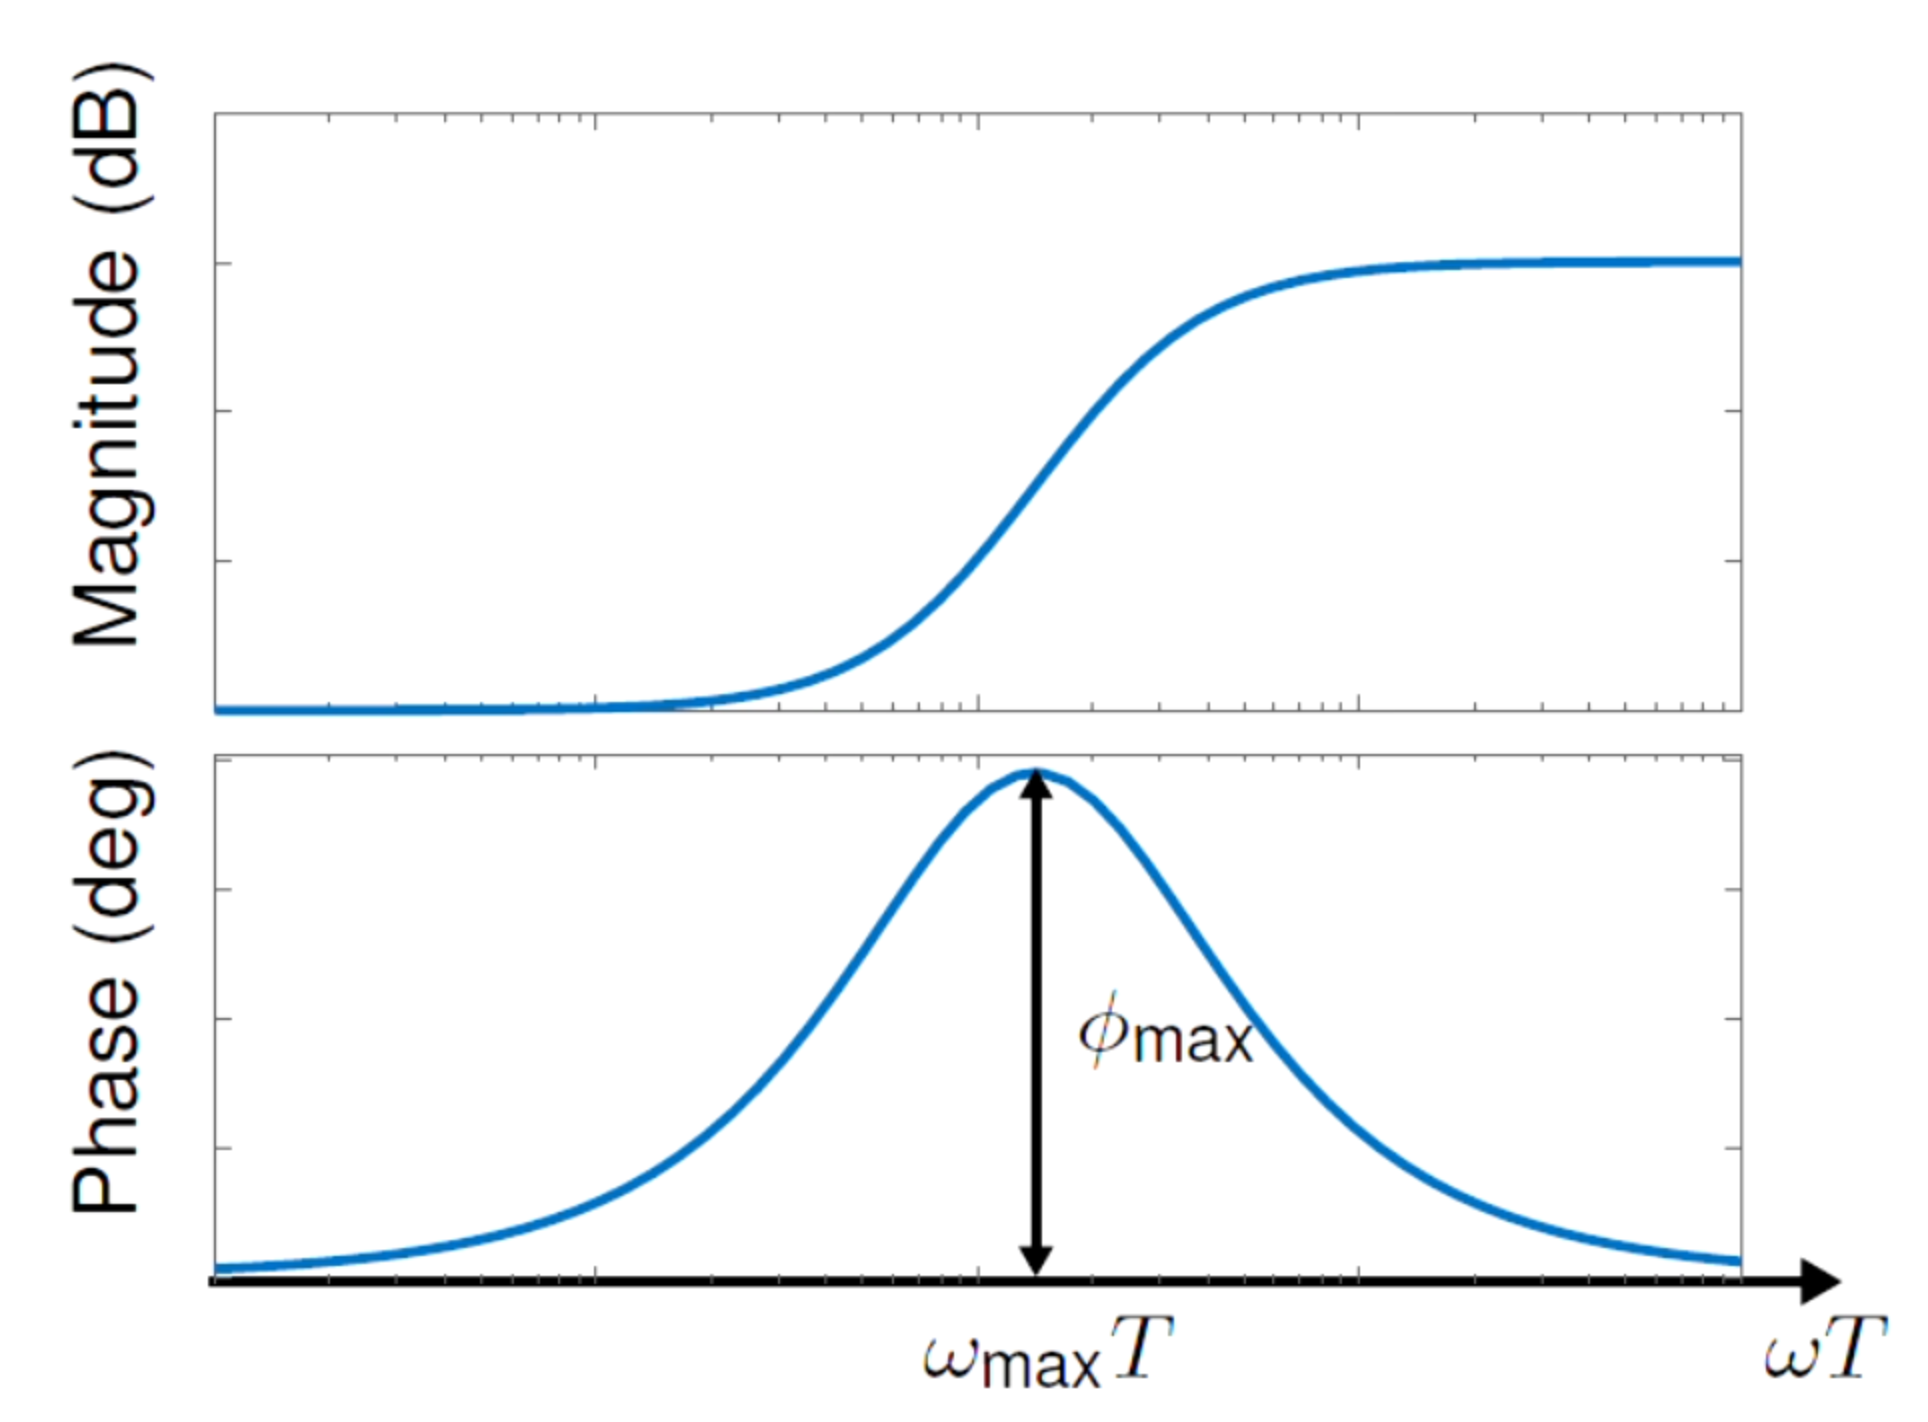
\includegraphics[width=0.5\textwidth]{Images/leadComp.png}
\end{center}

\subsubsection{Lag compensation}
A lag compensator can be used for minimizing the steady state error without affecting
the other dynamics. Only looking at stationary error. It doesn't eliminate the error
but reduces it.

For a lag compensator the pole comes before the zero.


A lag compensator can be written as:
$$D(s) = K_0 \frac{\alpha Ts+1}{\alpha Ts+1}$$
where $K_0$ is the gain of the compensator, $z>p \in \mathbb{R}$ and $\alpha > 1$.

The gain decreases and the phase gets negative.


\begin{center}
	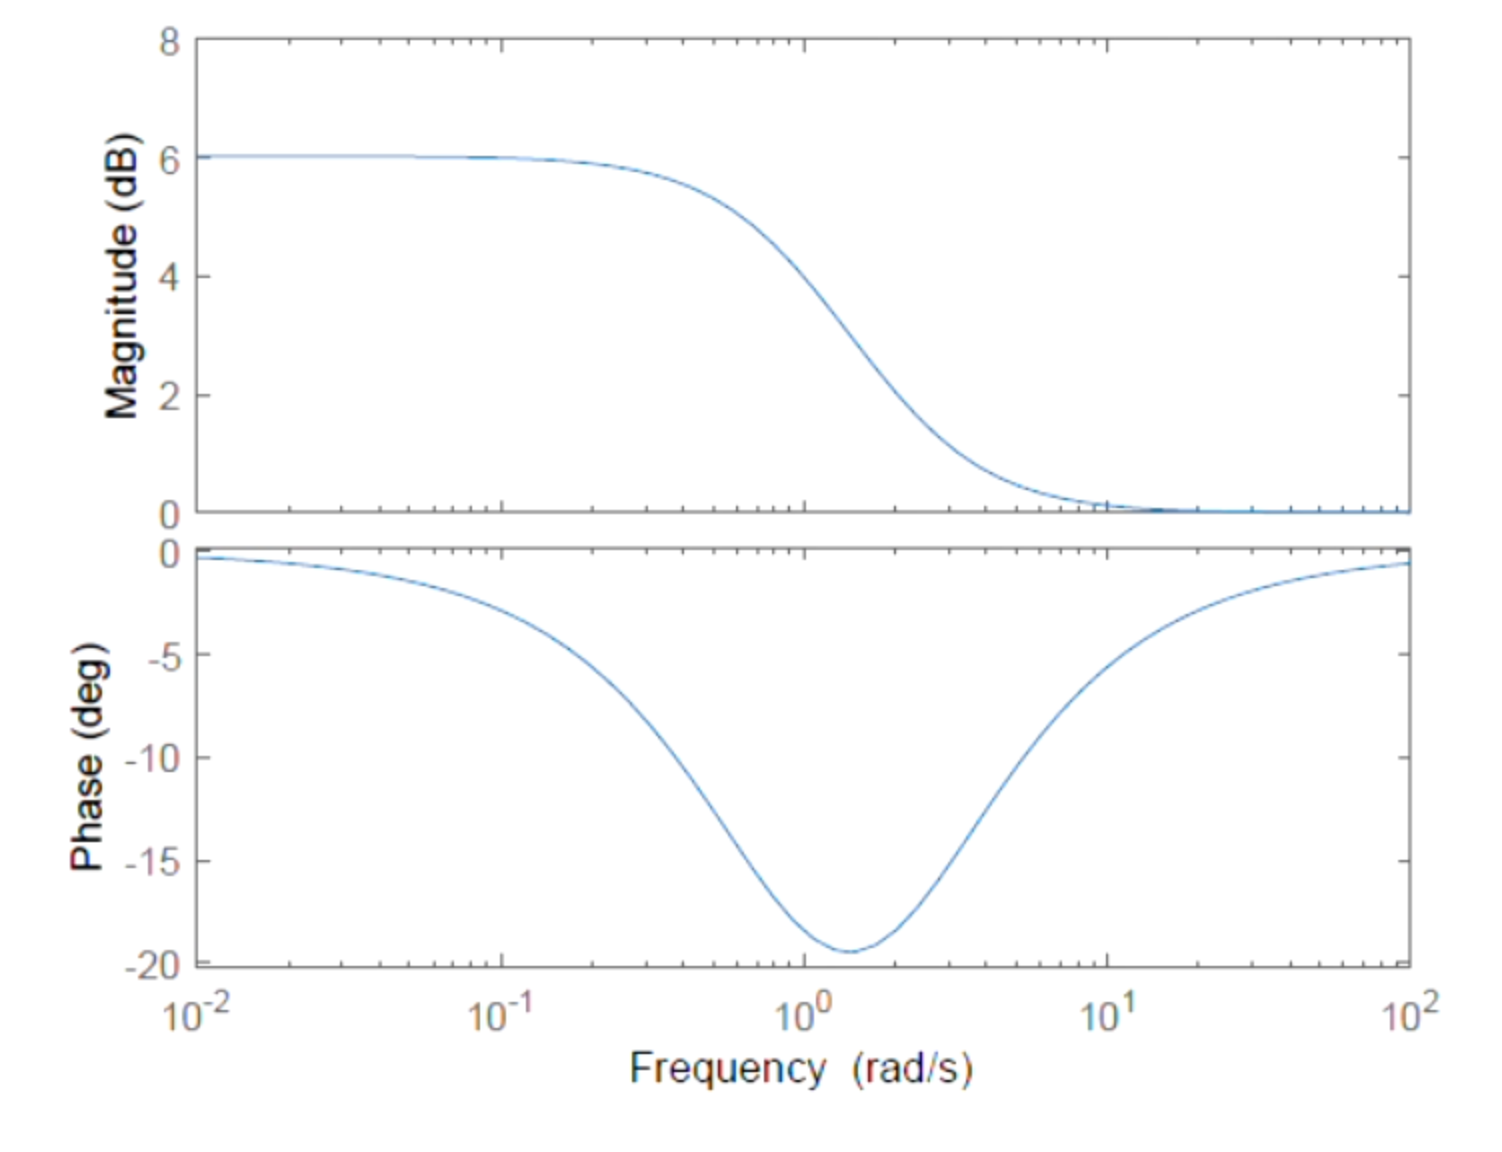
\includegraphics[width=0.5\textwidth]{Images/lagComp.png}
\end{center}

\subsection{Examples}

\textbf{Lead compensation}

Phase margin is found at 1.68 rad/s to be $7^\circ$.

To allow a phase margin of $25^\circ$ plus 10 for extra margin the needed phase lead is:
$$\phi_{max} = 25 + 10 - 7 = 28^\circ$$

The value of $\alpha$ is found by:
$$\alpha = \frac{1-sin(28)}{1+sin(28)} = 0.3610$$
Pick $\omega_{max}$ to be at the crossover frequency, i.e., $\omega_{max} = 1.68$ rad/s.
Then the value of $T$ is:

$$T = \frac{1}{\omega_{max}\sqrt{\alpha}} = 0.9906$$

Test the new system and verify. This shows that the phase margin is too small. Thus, you should reiterate by moving
the pole and zero.
